\chapter{Sprint 5 : Intelligence artificielle}

\section*{Introduction}
Le cinquième et dernier sprint livre la fonctionnalité différenciante de la plateforme :
un moteur d'IA hybride combinant un modèle de Machine Learning à 22 variables (ensemble
Gradient Boosting + Random Forest) pour la recommandation d'assignation, et un LLM
(Llama 3.3 70B via OpenRouter) pour l'estimation de durée, la détection de risques et
l'assistance conversationnelle.

% ============================================================
\section{Sprint Backlog}

\begin{table}[H]
  \centering
  \caption{Sprint Backlog — Sprint 5}
  \label{tab:backlog_s5}
  \begin{tabularx}{\textwidth}{C{1.2cm}L{5.5cm}L{2.5cm}C{2cm}C{1.5cm}}
    \toprule
    \thead{ID} & \thead{User Story} & \thead{Acteur} & \thead{Priorité} & \thead{Points} \\
    \midrule
    \rowcolor{lightgray}
    US-23 & Obtenir une recommandation ML d'assignation    & Member       & Must   & 13 \\
    US-24 & Estimer la durée d'une tâche par IA            & Member       & Must   &  8 \\
    \rowcolor{lightgray}
    US-25 & Discuter avec l'assistant IA                   & Member/Admin & Should &  8 \\
    US-26 & Relancer l'entraînement du modèle ML           & Admin        & Could  &  5 \\
    \midrule
    \multicolumn{4}{r}{\textbf{Total :}} & \textbf{34} \\
    \bottomrule
  \end{tabularx}
\end{table}

% ============================================================
\section{Conception}

\subsection{Diagramme de cas d'utilisation}

\begin{figure}[H]
  \centering
  \IfFileExists{figures/sprint5_use_case.png}{%
    \includegraphics[width=0.88\textwidth]{figures/sprint5_use_case.png}%
  }{%
    \fbox{\parbox{0.88\textwidth}{\centering\vspace{1.8cm}
      \textbf{[IMAGE A INSÉRER]}\\[0.4em]
      \texttt{figures/sprint5\_use\_case.png}\\[0.3em]
      \textit{Cas d'utilisation : Member, Admin, Service ML (FastAPI), LLM (OpenRouter)}
    \vspace{1.8cm}}}%
  }
  \caption{Diagramme de cas d'utilisation — Sprint 5}
  \label{fig:uc_s5}
\end{figure}

\subsection{Diagramme de séquence — Recommandation ML (12 étapes)}

\begin{figure}[H]
  \centering
  \IfFileExists{figures/sprint5_sequence_ml.png}{%
    \includegraphics[width=0.92\textwidth]{figures/sprint5_sequence_ml.png}%
  }{%
    \fbox{\parbox{0.92\textwidth}{\centering\vspace{2cm}
      \textbf{[IMAGE A INSÉRER]}\\[0.4em]
      \texttt{figures/sprint5\_sequence\_ml.png}\\[0.3em]
      \textit{Séquence ML : React → MLController → FastAPI → FeatureExtractor (22 feat.)
      → VotingClassifier → AiRecommendation → Response}
    \vspace{2cm}}}%
  }
  \caption{Diagramme de séquence — Pipeline de recommandation ML}
  \label{fig:seq_ml}
\end{figure}

\subsection{Diagramme de classes}

\begin{figure}[H]
  \centering
  \IfFileExists{figures/sprint5_class.png}{%
    \includegraphics[width=0.88\textwidth]{figures/sprint5_class.png}%
  }{%
    \fbox{\parbox{0.88\textwidth}{\centering\vspace{1.8cm}
      \textbf{[IMAGE A INSÉRER]}\\[0.4em]
      \texttt{figures/sprint5\_class.png}\\[0.3em]
      \textit{Classes : AiRecommendation, AIService, MLController, FastAPIRecommender, FeatureExtractor}
    \vspace{1.8cm}}}%
  }
  \caption{Diagramme de classes — Sprint 5}
  \label{fig:class_s5}
\end{figure}

\subsection{Les 22 variables du vecteur ML}

\begin{table}[H]
  \centering
  \caption{Variables du vecteur de features ML — réparties en 5 familles}
  \label{tab:features_ml}
  \begin{tabularx}{\textwidth}{C{1.5cm}L{3cm}X}
    \toprule
    \thead{Famille} & \thead{N° Features} & \thead{Description} \\
    \midrule
    \rowcolor{lightgray}
    Spécialités      & 1 -- 3  & Correspondance entre compétences requises et profil de l'utilisateur \\
    Charge actuelle  & 4 -- 6  & Nombre de tâches ouvertes, heures allouées, disponibilité restante \\
    \rowcolor{lightgray}
    Performance hist. & 7 -- 12 & Respect des délais, précision estimations, taux de réussite par type \\
    Familiarité ctx. & 13 -- 15 & Connaissance du projet, de l'équipe, du type de tâche \\
    \rowcolor{lightgray}
    Tendance \& collab. & 16 -- 22 & Vélocité récente, alignement sprint, qualité de collaboration \\
    \bottomrule
  \end{tabularx}
\end{table}

% ============================================================
\subsection{Collecte et préparation des données}

En l'absence d'un historique réel de projets au démarrage du PFE, un jeu de données
synthétiques a été généré avec la bibliothèque Python \textbf{Faker} et des
distributions statistiques cohérentes avec des profils de projets logiciels.

\begin{table}[H]
  \centering
  \caption{Composition du jeu de données d'entraînement}
  \label{tab:dataset_ml}
  \begin{tabularx}{\textwidth}{L{5cm}C{3cm}X}
    \toprule
    \thead{Ensemble} & \thead{Volume} & \thead{Description} \\
    \midrule
    \rowcolor{lightgray}
    Tâches simulées    & 8\,000      & Profils variés (priorité, complexité, type) \\
    Utilisateurs       & 50          & Spécialités, vélocités, historiques distincts \\
    \rowcolor{lightgray}
    Projets            & 20          & Durées de 4 à 52 semaines \\
    Assignations       & 24\,000     & Historique d'affectation et de performance \\
    \rowcolor{lightgray}
    Ratio positif/négatif & 42\,\%/58\,\% & Classes déséquilibrées — SMOTE appliqué \\
    \bottomrule
  \end{tabularx}
\end{table}

\subsection{Prétraitement des données}

Le pipeline de prétraitement (classe \texttt{FeatureExtractor}) effectue
les transformations suivantes avant toute inférence ou entraînement :

\begin{enumerate}
  \item \textbf{Encodage des variables catégorielles} : \texttt{priority},
        \texttt{task\_type}, \texttt{specialty} → encodage ordinal ou one-hot
        selon la cardinalité ;
  \item \textbf{Normalisation} : les features numériques (charge, heures, vélocité)
        sont standardisées (\texttt{StandardScaler}, $\mu=0$, $\sigma=1$) ;
  \item \textbf{Gestion des valeurs manquantes} : imputation par la médiane pour
        les features continues, par le mode pour les catégorielles ;
  \item \textbf{SMOTE} : sur-échantillonnage de la classe minoritaire (tâches
        en retard) pour équilibrer les classes dans le modèle de détection de risques ;
  \item \textbf{Sélection de features} : test $\chi^2$ et importance Gini pour
        réduire de 40 à 22 les features retenues (seuil d'importance $> 0.01$).
\end{enumerate}

\subsection{Entraînement des modèles}

Trois algorithmes ont été évalués pour chacune des deux tâches ML :

\begin{table}[H]
  \centering
  \caption{Algorithmes évalués par tâche ML}
  \label{tab:algos_ml}
  \begin{tabularx}{\textwidth}{L{5cm}L{3.5cm}X}
    \toprule
    \thead{Tâche} & \thead{Algorithme} & \thead{Hyperparamètres principaux} \\
    \midrule
    \rowcolor{lightgray}
    Recommandation d'assignation  & GBM (retenu)       & \texttt{n\_estimators=200, max\_depth=5, lr=0.05} \\
    Recommandation d'assignation  & Random Forest      & \texttt{n\_estimators=150, max\_depth=8} \\
    \rowcolor{lightgray}
    Recommandation d'assignation  & Régression log.    & Baseline linéaire \\
    Estimation de durée           & Random Forest (retenu) & \texttt{n\_estimators=200, max\_depth=10} \\
    \rowcolor{lightgray}
    Estimation de durée           & GBM                & \texttt{n\_estimators=200, lr=0.05} \\
    Estimation de durée           & Régression linéaire & Baseline linéaire \\
    \bottomrule
  \end{tabularx}
\end{table}

La recherche d'hyperparamètres a utilisé \textbf{GridSearchCV} avec une
validation croisée à 5 plis (\texttt{StratifiedKFold} pour la classification,
\texttt{KFold} pour la régression). L'optimisation a ciblé l'AUC ROC pour la
détection de risques et le MAE pour l'estimation de durée.

\subsection{Évaluation des performances}

\begin{table}[H]
  \centering
  \caption{Résultats complets — Modèle de recommandation d'assignation (AUC ROC)}
  \label{tab:eval_recommandation}
  \begin{tabularx}{\textwidth}{L{5cm}C{2.5cm}C{2.5cm}C{2.5cm}C{2cm}}
    \toprule
    \thead{Algorithme} & \thead{Accuracy} & \thead{F1-score} & \thead{AUC ROC} & \thead{Temps (ms)} \\
    \midrule
    \rowcolor{lightgray}
    \textbf{GBM (retenu)} & \textbf{0,89} & \textbf{0,85} & \textbf{0,92} & 12,1 \\
    Random Forest         & 0,86          & 0,82          & 0,89          & 8,4 \\
    \rowcolor{lightgray}
    Régression logistique & 0,79          & 0,72          & 0,82          & 0,3 \\
    \bottomrule
  \end{tabularx}
\end{table}

La matrice de confusion du modèle GBM retenu montre un \textbf{rappel de 0,88}
sur la classe « tâche à risque » : seuls 12\,\% des cas à risque réel ne sont pas
détectés. Ce compromis précision/rappel est jugé acceptable pour un contexte de
recommandation assistée (l'utilisateur reste maître de la décision finale).

\subsection{Déploiement du modèle ML}

Les modèles entraînés sont sérialisés au format \textbf{Joblib} et chargés en
mémoire au démarrage du microservice FastAPI, éliminant le coût de désérialisation
à chaque requête. L'architecture de déploiement du microservice est la suivante :

\begin{lstlisting}[style=yamlstyle,caption={Structure du microservice FastAPI},
  label={lst:fastapi_structure}]
ml-service/
  app/
    main.py            # FastAPI app, /recommend, /estimate, /risk
    feature_extractor.py   # 22 features pipeline
    models/
      voting_clf.joblib  # GBM + RF VotingClassifier
      rf_duration.joblib # Random Forest regression
      scaler.joblib      # StandardScaler fitted
  requirements.txt
  Dockerfile           # python:3.11-slim, uvicorn
\end{lstlisting}

Le microservice expose trois endpoints REST authentifiés par clé API partagée
avec le backend Laravel. En cas d'indisponibilité du service ML, Laravel renvoie
une réponse dégradée (HTTP 503) avec un message d'erreur explicite, préservant
ainsi la disponibilité de l'application principale.

% ============================================================
\section{Réalisation}

\subsection{Page IA et analyses}

\begin{figure}[H]
  \centering
  \IfFileExists{figures/sprint5_22_ai_home.png}{%
    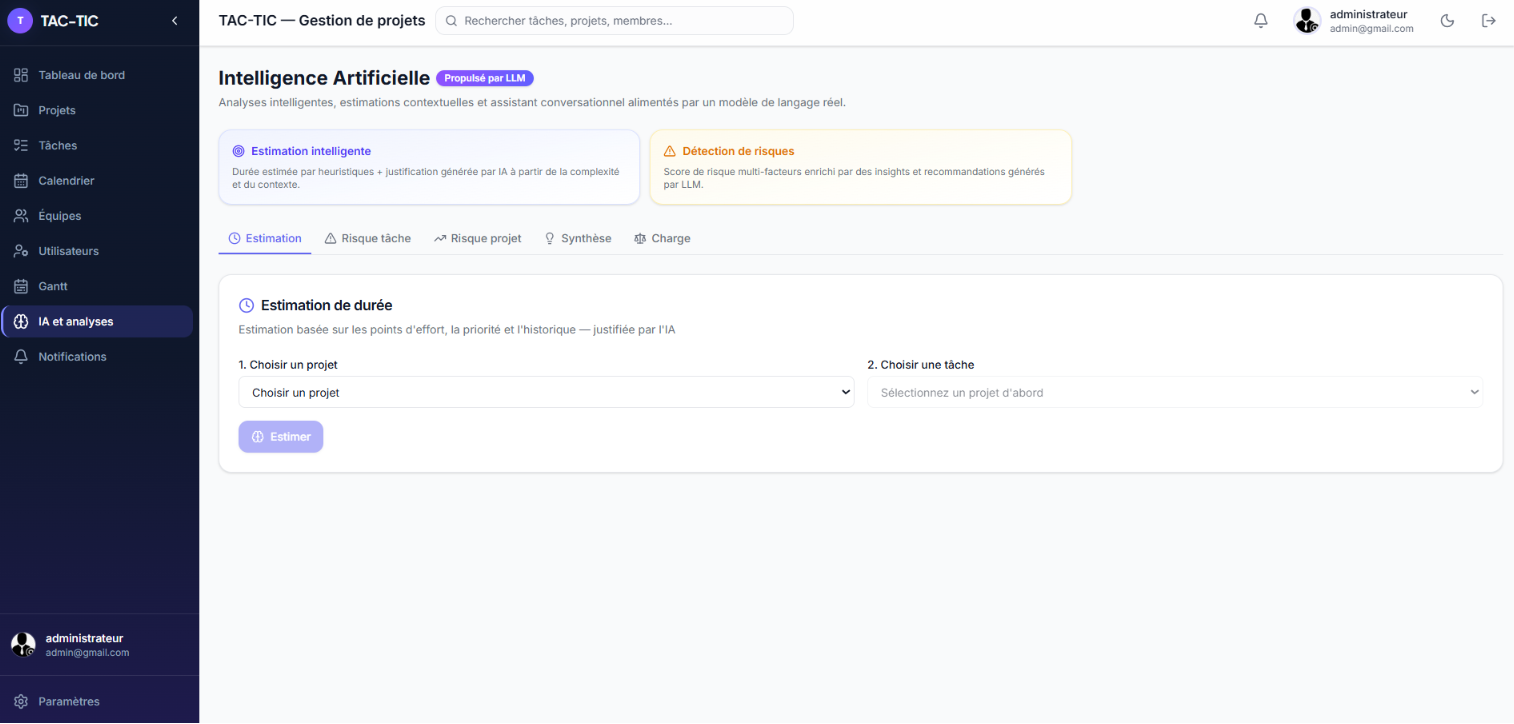
\includegraphics[width=0.88\textwidth]{figures/sprint5_22_ai_home.png}%
  }{%
    \fbox{\parbox{0.88\textwidth}{\centering\vspace{2cm}
      \textbf{[IMAGE A INSÉRER]}\\[0.4em]
      \texttt{figures/sprint5\_22\_ai\_home.png}\\[0.3em]
      \textit{Page IA : badge «~Propulsé par LLM~», cartes Estimation / Détection de risques, 5 onglets}
    \vspace{2cm}}}%
  }
  \caption{Page Intelligence Artificielle — Vue principale}
  \label{fig:ui_ai_home}
\end{figure}

\subsection{Résultat d'estimation IA}

\begin{figure}[H]
  \centering
  \IfFileExists{figures/sprint5_23_ai_estimate.png}{%
    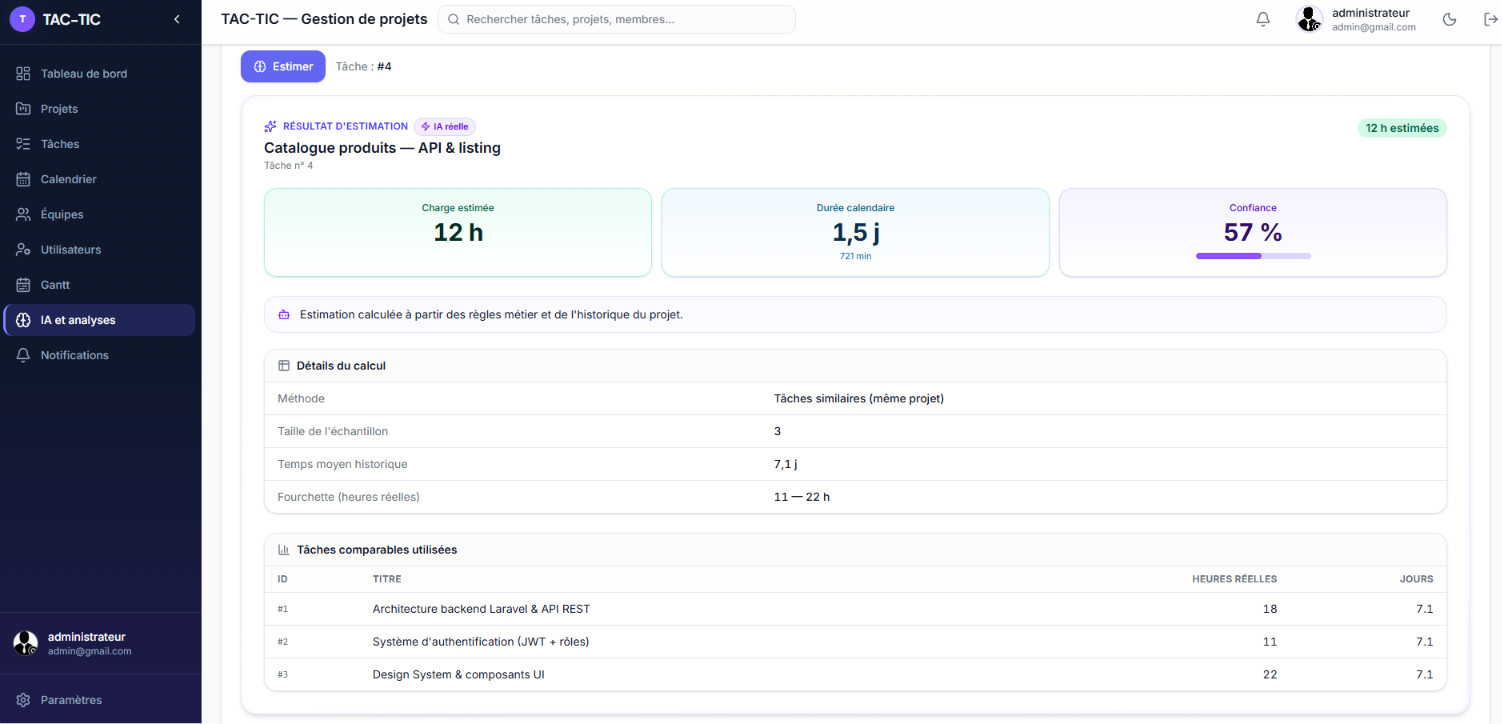
\includegraphics[width=0.85\textwidth]{figures/sprint5_23_ai_estimate.png}%
  }{%
    \fbox{\parbox{0.85\textwidth}{\centering\vspace{2cm}
      \textbf{[IMAGE A INSÉRER]}\\[0.4em]
      \texttt{figures/sprint5\_23\_ai\_estimate.png}\\[0.3em]
      \textit{Estimation «~Architecture backend Laravel~» : 9,8h / 1,2j / confiance 57\,\%
      + justification LLM}
    \vspace{2cm}}}%
  }
  \caption{Résultat d'estimation de durée par LLM}
  \label{fig:ui_ai_estimate}
\end{figure}








% ============================================================
\section{Tests unitaires et validation expérimentale}

\begin{lstlisting}[style=phpstyle,caption={Tests unitaires Laravel — MLController},label={lst:tests_s5_php}]
it('returns 503 when ML service is unavailable', function () {
    Http::fake(['*' => Http::response(null, 503)]);
    $task = Task::factory()->create();
    $this->actingAs($task->project->owner)
         ->getJson("/api/ml/recommend/{$task->id}")
         ->assertStatus(503)
         ->assertJson(['error' => 'ml_unavailable']);
});
\end{lstlisting}

\begin{lstlisting}[style=pythonstyle,caption={Tests unitaires Python — FastAPI},label={lst:tests_s5_py}]
def test_recommend_returns_ranked_candidates():
    r = TestClient(app).post('/recommend', json={
        'title': 'API module', 'priority': 'high',
        'story_points': 8, 'complexity': 6,
        'required_specialties': ['Backend'], 'project_id': 1
    })
    assert r.status_code == 200
    cands = r.json()
    assert len(cands) > 0
    # Les candidats doivent être triés par score décroissant
    assert cands[0]['score'] >= cands[-1]['score']
\end{lstlisting}

\subsection{Validation expérimentale des modèles}

\begin{table}[H]
  \centering
  \caption{Validation du modèle d'estimation de durée (80/20 split, 8\,000 tâches)}
  \label{tab:valid_duree}
  \begin{tabularx}{\textwidth}{L{4.5cm}C{2.5cm}C{2.5cm}C{2cm}C{2.5cm}}
    \toprule
    \thead{Algorithme} & \thead{MAE (h)} & \thead{RMSE (h)} & \thead{R²} & \thead{Inférence (ms)} \\
    \midrule
    \rowcolor{lightgray}
    \textbf{Random Forest (retenu)} & \textbf{1,42} & \textbf{2,18} & \textbf{0,82} & 8,4 \\
    GBM Scikit-learn & 1,68 & 2,54 & 0,76 & 12,1 \\
    \rowcolor{lightgray}
    Régression linéaire & 3,21 & 4,67 & 0,51 & 0,3 \\
    \bottomrule
  \end{tabularx}
\end{table}

\begin{table}[H]
  \centering
  \caption{Validation du modèle de détection de risques}
  \label{tab:valid_risque}
  \begin{tabularx}{\textwidth}{L{4.5cm}C{3cm}C{3cm}C{3cm}}
    \toprule
    \thead{Algorithme} & \thead{Accuracy} & \thead{F1-score} & \thead{AUC ROC} \\
    \midrule
    \rowcolor{lightgray}
    \textbf{GBM Scikit-learn (retenu)} & \textbf{0,89} & \textbf{0,85} & \textbf{0,92} \\
    Random Forest & 0,86 & 0,82 & 0,89 \\
    \rowcolor{lightgray}
    Régression logistique & 0,79 & 0,72 & 0,82 \\
    \bottomrule
  \end{tabularx}
\end{table}

\begin{chapconclusion}
Le sprint~5 livre la fonctionnalité la plus différenciante du PFE — un moteur IA
hybride opérationnel intégré nativement dans le workflow de création de tâches.
Les métriques de validation confirment la qualité des choix algorithmiques :
AUC ROC de 0,92 pour la détection de risques et MAE de 1,42\,h pour l'estimation
de durée. Le microservice FastAPI répond en moins de 45\,ms (médiane P50), bien en
dessous du seuil d'acceptabilité de 500\,ms. Le pipeline ML complet (collecte,
prétraitement, entraînement, évaluation, déploiement Joblib) est reproductible et
prêt pour un réentraînement sur des données réelles en production.
\end{chapconclusion}
